\section{سوال دوم}

۵ مثال از سیستم‌های کامپیوتری بزنید و در هرکدام \lr{Fault} و \lr{Error} و \lr{Failure} را مشخص کنید.


\begin{qsolve}[]
	\begin{enumerate}
		\item 
		\textbf{الگوریتم}\\
		برنامه زیر را درنظر بگیرید:
\begin{latin}
\begin{lstlisting}[language=C++]
int a;
a = cin >> "Enter_number:";
if(a > 10)
   cout << "True!" << endl;
else
   cout << "False!" << endl;
\end{lstlisting} 
\end{latin}

‫در‬‫اینجا‬ ‫فرض‬ ‫کنیم‬ ‫کاربر‬ ‫عدد‬ ‫‪۱۰‬‬ ‫را‬ ‫وارد‬ ‫کند‬ ‫و‬ ‫طبق‬ ‫الگوریتم‬ ‫تعریف‬ ‫شده‬ ‫برای‬ ‫مسئله‬ ‫انتظار‬ ‫می‬ ‫رود‬ ‫خروجی \lr{\texttt{True!}} باشد. درحالی که در برنامه نوشته شده خروجی \lr{\texttt{False!}} چاپ می‌شود.

	
	\begin{itemize}
		\item \lr{\textbf{:Fault}}\\
		اشکال به دلیل عدم دقت برنامه‌نویس در نوشتن شرط \texttt{if} به وجود آمده است. (نگذاشتن شرط بزرگ‌تر مساوی و قراردادن شرط بزرگ‌تر به‌جای آن)
		
		\item \lr{\textbf{:Error}}\\
		اجرای نادرست و اشتباه \texttt{else}. به دلیل رخ‌دادن اشکال در نوشتن کد، بخشی از کد که موردنظر ما نبوده اجرا می‌شود.
		
		\item \lr{\textbf{:Failure}}\\
		نشان‌دادن خروجی نادرست به کاربر.
	\end{itemize}
	
	
	
	
	\item 
	\textbf{پرتوهای کیهانی}\\
	قطع شارژ سلول‌های \lr{DRAM} موجود در یک حافظه بر اثر تابش پرتو‌های کیهانی.
	
	\begin{itemize}
		\item \lr{\textbf{:Fault}}\\
		برخورد پرتو‌های کیهانی به حافظه.
		
		\item \lr{\textbf{:Error}}\\
		فلیپ شدن بیت‌های حافظه.
		
		\item \lr{\textbf{:Failure}}\\
		انجام محاسبات اشتباه بر اثر فیلیپ شدن بیت‌ها.
	\end{itemize}
	
	
	
	\item 
	\textbf{حمله ویروس به کامپیوتر}\\
	فرض کنید در حین استفاده از اینترنت، یک فایل آلوده به ویروس را دانلود کرده‌اید و متوجه آن نشده‌اید.
	
	\begin{itemize}
		\item \lr{\textbf{:Fault}}\\
		ویروس به بخشی از فایل‌های سیستم شما نفوذ می‌کند و برخی از فایل‌های مهم سیستم‌عامل یا برنامه‌ها را تخریب می‌کند.
		
		\item \lr{\textbf{:Error}}\\
		سیستم شما شروع به نشان دادن رفتارهای غیرعادی می‌کند؛ برنامه‌ها به درستی باز نمی‌شوند یا خطاهای ناگهانی رخ می‌دهد. ممکن است پیغام‌های خطای ناگهانی ظاهر شوند یا برنامه‌ها متوقف شوند.
	\end{itemize}
	\end{enumerate}
\end{qsolve}



\begin{qsolve}
	\begin{enumerate}
		\item [ ]
		\begin{itemize}
			\item \lr{\textbf{:Failure}}\\
			در نهایت، ویروس به قدری سیستم شما را تخریب می‌کند که سیستم کاملاً غیرقابل استفاده می‌شود و حتی ممکن است فایل‌های مهم شما پاک شوند. سیستم باید مجدداً از اول نصب شود یا نیاز به بازیابی داده‌ها دارید.
		\end{itemize}
		
		\item [4.]
		\textbf{خرابی شبکه در شرکت}\\
		فرض شود در یک شرکت مشغول کار هستید و همه کامپیوترها به یک شبکه داخلی متصل هستند که به سرور مرکزی دسترسی دارند.
		
		\begin{itemize}
			\item \lr{\textbf{:Fault}}\\
			یکی از روترهای شبکه به دلیل نوسان برق دچار نقص می‌شود و دیگر نمی‌تواند داده‌ها را به درستی به سرور مرکزی ارسال کند. نوسان برق به‌عنوان \lr{Fault} انتخاب می‌شود.
			
			\item \lr{\textbf{:Error}}\\
			به دلیل خرابی روتر، ارتباط بین برخی از کامپیوترها و سرور مرکزی قطع می‌شود و کاربران نمی‌توانند به فایل‌ها و داده‌های موجود روی سرور دسترسی پیدا کنند.
			
			\item \lr{\textbf{:Failure}}\\
			در نهایت، شبکه به طور کامل از کار می‌افتد و هیچ‌یک از کاربران نمی‌توانند به سرور یا اینترنت دسترسی پیدا کنند تا زمانی که روتر تعمیر یا تعویض شود.
		\end{itemize}
		
		
		\item [5.]
		\textbf{مدارمنطقی}\\
		سناریو مقابل را درنظر بگیرید: یک مقایسه‌کننده ۲ بیتی نوشته ام که دو عدد ۲ بیتی $a$ و $b$ را مقایسه می‌کند. فرض کنیم:‌ 
		\begin{center}
			\begin{latin}
				$a=a_1a_0$\\
				$b=b_1b_0$ 
			\end{latin} 
		\end{center}
		
		
		با استفاده از جدول درستی و حدول کارنو خروجی مطلوب ما در این مسئله یعنی بزرگتر بودن $a$ نسبت به $b$ به‌صورت مقابل خواهد بود:
		\begin{center}
			\begin{latin}
				$F=a_1b'_1 + a_0b'_1b'0 + a_1a_0b'_0$
			\end{latin}
		\end{center}
	\end{enumerate}
\end{qsolve}



\begin{qsolve}
	\begin{enumerate}
		\item [ ]
		
		\begin{center}
			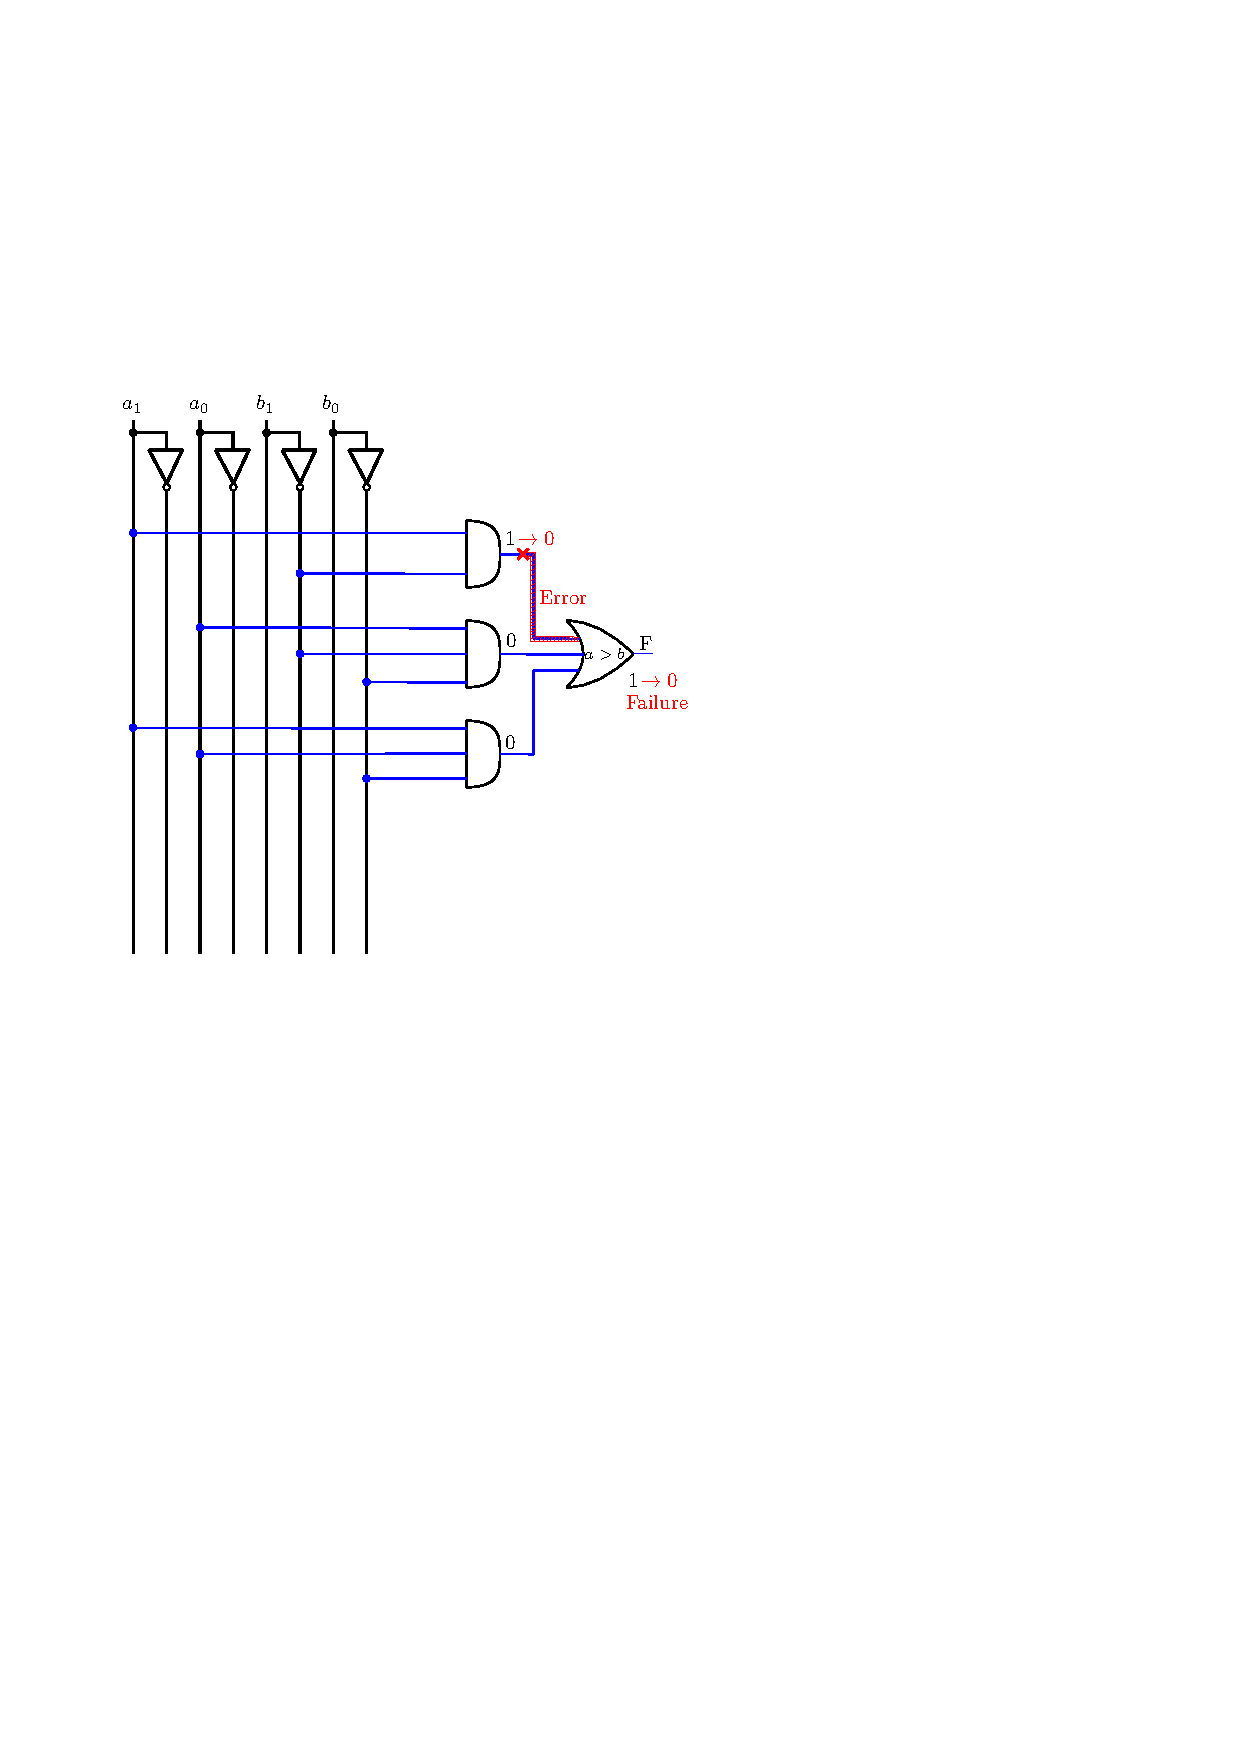
\includegraphics[width=12cm]{pics/comp.pdf}
		\end{center}
		
		با فرض اینکه مقدار ورودی‌ها $a=10$ و $b=01$ باشد، خروجی در حالت درست باید ۱ باشد ولی به‌دلیل رخ‌دادن "اشکال چسبیده به صفر" خروجی صفر می‌شود.
		
		
		
		\item \lr{\textbf{:Fault}}\\
		وجود اشکال "چسبیده به صفر" (اشکال دائم)
		
		\item \lr{\textbf{:Error}}\\
		انتشار مقدار نادرست از خروجی \lr{AND} (مسیر آلوده شده که با رنگ قرمز در شکل نشان داده شده است، بیانگر مسیر انتشار \lr{Error} است)
		
		\item \lr{\textbf{:Failure}}\\
		نمایش خروجی نادرست (عدم تشخیص بزرگ‌تر بودن $a$ نسبت به $b$)
		
	\end{enumerate}
\end{qsolve}




